%%
% このファイルは、筑波大学情報学群情報科学類の
% 卒業研究論文本体のサンプルです。
% このファイルを書き換えて、この例と同じような書式の論文本体を
% LaTeXを使って作成することができます。
%
% PC環境や、LaTeX環境の設定によっては漢字コードや改行コードを
% 変更する必要があります。
%%
\documentclass[a4paper,11pt]{jreport}

%%【PostScript, JPEG, PNG等の画像の貼り込み】
%% 利用するパッケージを選んでコメントアウトしてください。
%\usepackage{graphicx} % for \includegraphics[width=3cm]{sample.eps}
\usepackage[dvipdfmx]{graphicx, color}
%\usepackage{epsfig} % for \psfig{file=sample.eps,width=3cm}
%\usepackage{epsf} % for \epsfile{file=sample.eps,scale=0.6}
%\usepackage{epsbox} % for \epsfile{file=sample.eps,scale=0.6}

%% dvipdfm を使う場合(dvi->pdfを直接生成する場合)
%\usepackage[dvipdfmx]{color}
%% dvipdfm を使ってPDFの「しおり」を付ける場合
%\usepackage[dvipdfm,bookmarks=true,bookmarksnumbered=true,bookmarkstype=toc]{hyperref}
%% 参考:dvipdfm 日本語版
%% http://hamilcar.phys.kyushu-u.ac.jp/~hirata/dvipdfm/
\usepackage[left=25truemm,top=35truemm,right=25truemm,bottom=50truemm]{geometry}
\usepackage{times} % use Times Font instead of Computer Modern

\setcounter{tocdepth}{3}
\setcounter{page}{-1}

\setlength{\parskip}{0em}
\setlength{\topsep}{0em}

%\newcommand{\zu}[1]{{\gt \bf 図\ref{#1}}}

%% タイトル生成用パッケージ(重要)
\usepackage{coins-jp-utf8}

\usepackage{siunitx}
\usepackage{amsmath}
\usepackage[margin=5pt]{subcaption}
% !TEX root = ../interaction2017_shima.tex

% 手法名
\newcommand{\SysName}{本プロトタイプ}
\newcommand{\selection}{選択ジェスチャ}
\newcommand{\operation}{操作ジェスチャ}

% 修正とTODO
\newcommand{\fixme}[1]{\textcolor[rgb]{1,0,0}{#1}}
\newcommand{\TODO}[1]{\textcolor[rgb]{0,0,1}{#1}}
%本番は↓のコメントアウトを外すこと!!!
%\renewcommand{\TODO}[1]{} \renewcommand{\fixme}[1]{}

% 参照
\newcommand{\refImg}[1]{図\ref{img:#1}}
\newcommand{\refSec}[1]{\ref{sec:#1}節}
\newcommand{\refSubsec}[1]{\ref{ssec:#1}項}
\newcommand{\refCha}[1]{第\ref{cha:#1}章}
\newcommand{\refEq}[1]{式\ref{eq:#1}}
%\newcommand{\refSec}[1]{第\ref{sec:#1}節}
\newcommand{\secLabel}[1]{\label{sec:#1}}
\newcommand{\subsecLabel}[1]{\label{ssec:#1}}
\newcommand{\chaLabel}[1]{\label{cha:#1}}

% 画像
\newcommand{\img}[5]{
\begin{figure}[#1]
	\begin{center}
		\includegraphics[width = #2\hsize]{./img/#3}
	\end{center}
	\caption{#4}
	\label{img:#5}
\end{figure}
}

% 複数コラムある場合のぶち抜き画像
\newcommand{\IMG}[5]{
\begin{figure*}[#1]
	\begin{center}
		\includegraphics[width = #2\hsize]{./img/#3}
	\end{center}
	\caption{#4}
	\label{img:#5}
\end{figure*}
}

\newcommand{\unit}[1]{\,#1} % 120,\unit{mm}→120mm」をイイ!感じにスペーシングしてくれる
\newcommand{\kake}{~$\times$~} % →×

% 情報処理学会のbibtexスタイル(ipsjunsrt.bstなど)を使うときにこれがないと,\newblockが定義されてないよってエラーになる
% 参考:http://gaso.hatenablog.com/entry/2014/05/11/%E6%9F%90%E5%AD%A6%E4%BC%9A%E3%83%86%E3%83%B3%E3%83%97%E3%83%AC%E3%81%AE%E3%82%B9%E3%82%BF%E3%82%A4%E3%83%AB%E3%83%95%E3%82%A1%E3%82%A4%E3%83%AB%E3%81%A7BibTeX%E3%82%92%E4%BD%BF%E3%81%A3%E3%81%9F%E6%99%82
\def\newblock{\hskip .11em plus .33em minus .07em}




%%
\newcommand{\iic}{\text{I}$^\text{2}$\text{C}}


%% タイトル
%% 【注意】タイトルの最後に\\ を入れるとエラーになります
%\title{密閉容器における受動音響センシングによる内容量推定}
\multilinetitle{距離センサを用いた膝の動きによるカーソル操作手法}
%% 著者
\author{市川 佑}
%% 指導教員
\advisor{高橋伸\ \ 志築文太郎}

%% 専攻名 と 年月 (提出年月)
%% 年月は必要に応じて書き替えてください。
\heiseiyear{30}  % 平成の年度
%\majorfield{ソフトウェアサイエンス主専攻}
\majorfield{情報システム主専攻}
%\majorfield{知能情報メディア主専攻}

\begin{document}
\maketitle
\thispagestyle{empty}
\newpage

\thispagestyle{empty}
\vspace*{20pt plus 1fil}
\parindent=1zw
\noindent
%%
%% 論文の概要(Abstract)
%%
\begin{center}
{\Large \bf 要  旨}
\vspace{2cm}
\end{center}
本研究では、\fixme{デスクトップ環境下において}

%%%%%
\par
\vspace{0pt plus 1fil}
\newpage

\pagenumbering{roman} % I, II, III, IV
\tableofcontents
\listoffigures
\listoftables

\pagebreak \setcounter{page}{1}
\pagenumbering{arabic} % 1,2,3

\chapter{序論}

\section{背景}
パーソナルコンピュータ、スマートフォン、タブレット端末に代表される情報端末が普及し、それらの操作方法は多岐にわたる。一般的に、パーソナルコンピュータはマウスやタッチパッドなどを用い、スマートフォン、タブレット端末においてはタッチパネルを搭載しており、直接触れることで、コンテンツを選択することができる。しかし、これらの操作方法は手を用いることを前提としており、特にパーソナルコンピュータの操作においてはキーボードも同時に用いるため、マウスと同時に操作することはできない。こうした問題を解決するために、手を用いない操作手法が多数提案されている。\\
\\
\TODO{視線や音声など、具体的に挙げる}\\
\\
本研究では、通常パーソナルコンピュータの使用には関わらない、足を用いた操作手法に着目する。具体的には、足をマウス操作に用いることで、上記の問題の解決をはかる。
\\
\\
\TODO{従来研究では足に何かを装着しなければならない点を挙げる}




\section{目的・アプローチ}


\section{貢献}
\section{本論文の構成}

\chapter{関連研究}

\section{足を入力操作として用いる研究}
Alexanderら\cite{Alexander:2012:PYB:2207676.2208575}は、モバイルデバイスのコマンドに対し、足によるジェスチャをマッピングするためのユーザ導出型の調査を行なった。
Felberbaumら\cite{Felberbaum:2018:BUF:3173574.3173908}は、立った状態、座った状態、投影された画面の上にいる状態の3条件で、GUIに関する操作、仮想空間に関する操作の2種類に対するジェスチャマッピングを調査した。この調査の中ではまた、ジェスチャと操作の対応が一意的かを表す指標を導入し評価を行なった。
鈴木\cite{ssuzuki_2009}は、測域センサを用いることで、足の動きをセンシングし、床面におけるインタラクション手法を提案している。
奥村\cite{okumura_2011}は、靴に加速度と角速度を取得することができるセンサを取り付け、外出時におけるモバイル端末の操作を行うシステムを開発した。

\section{足をポインタ操作として用いる研究}
足をポインタ操作に用いる研究は、1960年代から行われている。Englishら\cite{1698228}は、テキスト選択においていくつかの膝を含めた装置やデバイスを用いた時の操作時間を調査した。調査の結果、膝による操作は最も短い時間で選択することができることがわかった。

Pearsonら\cite{Pearson:1986:MMD:22627.22392, Pearson:1988:EET:49108.1046356}は「モル」という装置を開発し、ポインタの操作などに手の代わりに足を使用する方法を探索した。モルを用いた場合でも、訓練によって小さなターゲットを選択することが可能になることを示した。


近年でも、調査が行われている。Vellosoら\cite{velloso:hal-01599657}は、座っている状態の机の下の足の動きの特徴を調査した。この論文の中で、机の下に配置したトラッキングシステムから、片方の足のつま先をマウス操作に割り当て、1次元と2次元におけるポインティング作業により、パフォーマンスのテストを行なっている。
田中ら\cite{110004704997}は、足の指をマウス操作に用いるために、母指の力制御と運動特性を調査した。
Horodniczyら\cite{Horodniczy:2017:FHE:3025453.3025625}は、靴底に可変摩擦式の装置を取り付け、足をマウス操作に用いることを実現した。靴底には低摩擦材料と高摩擦材料の2つを取り付け、高摩擦材料の位置を制御することで、かかと部分の摩擦力を調整している。結果、2次元のポインティングタスクでエラー率においてマウスより優れた結果を発表した。
\section{\TODO{もう少し話を広げたい、背景次第ではあるが、カーソル操作の話か、それとも他の話か}}






\chapter{設計}
\section{概要}


\chapter{実装}
\section{概要}
\SysName は、ハードウェアとして三角法を用いた光学式距離センサ10個を一列に並べたセンサアレイと、センサから取得した値の処理と値を元に座標を計算するソフトウェアからなる。
\section{プロトタイプ1} 
\secLabel{proto1}
\subsection{ハードウェア}
距離センサはSHARP GP2Y0E03\footnote{http://www.sharp.co.jp/products/device/lineup/selection/opto/haca/diagram2.html}を使用した。この距離センサは三角測量の原理を用い、対象までの距離を計測する。本センサの値の取得には、Arduino MEGA 2560を用いる。距離センサとは\iic を用いて接続を行う。個々のセンサは、スレーブアドレスが初期値(0x40)で統一されているために、アプリケーションノート\footnote{http://www.sharp.co.jp/products/device/doc/opto/gp2y0e02\_03\_appl\_j.pdf}に記載されているe-fuseプログラミングの手順で、スレーブアドレスの変更を行なっている。これにより、10個の距離センサを2本の信号線で制御する。
接続した距離センサは1列に並べる。\SysName では、長さ約30\si{cm}のプラスティック製の定規を用意し、両面テープでセンサ本体を固定し、配線類をセロハンテープで固定した。装置が長細いため、接続にはブレッドボードの電源とグランド接続に用いられる部分を2列使用した。\refImg{ig1}は実際に製作したプロトタイプの1つである。\refImg{ig1}ではセンサごとの間隔は約11\si{mm}としている。
\begin{figure}[htbp]
	\begin{center}
		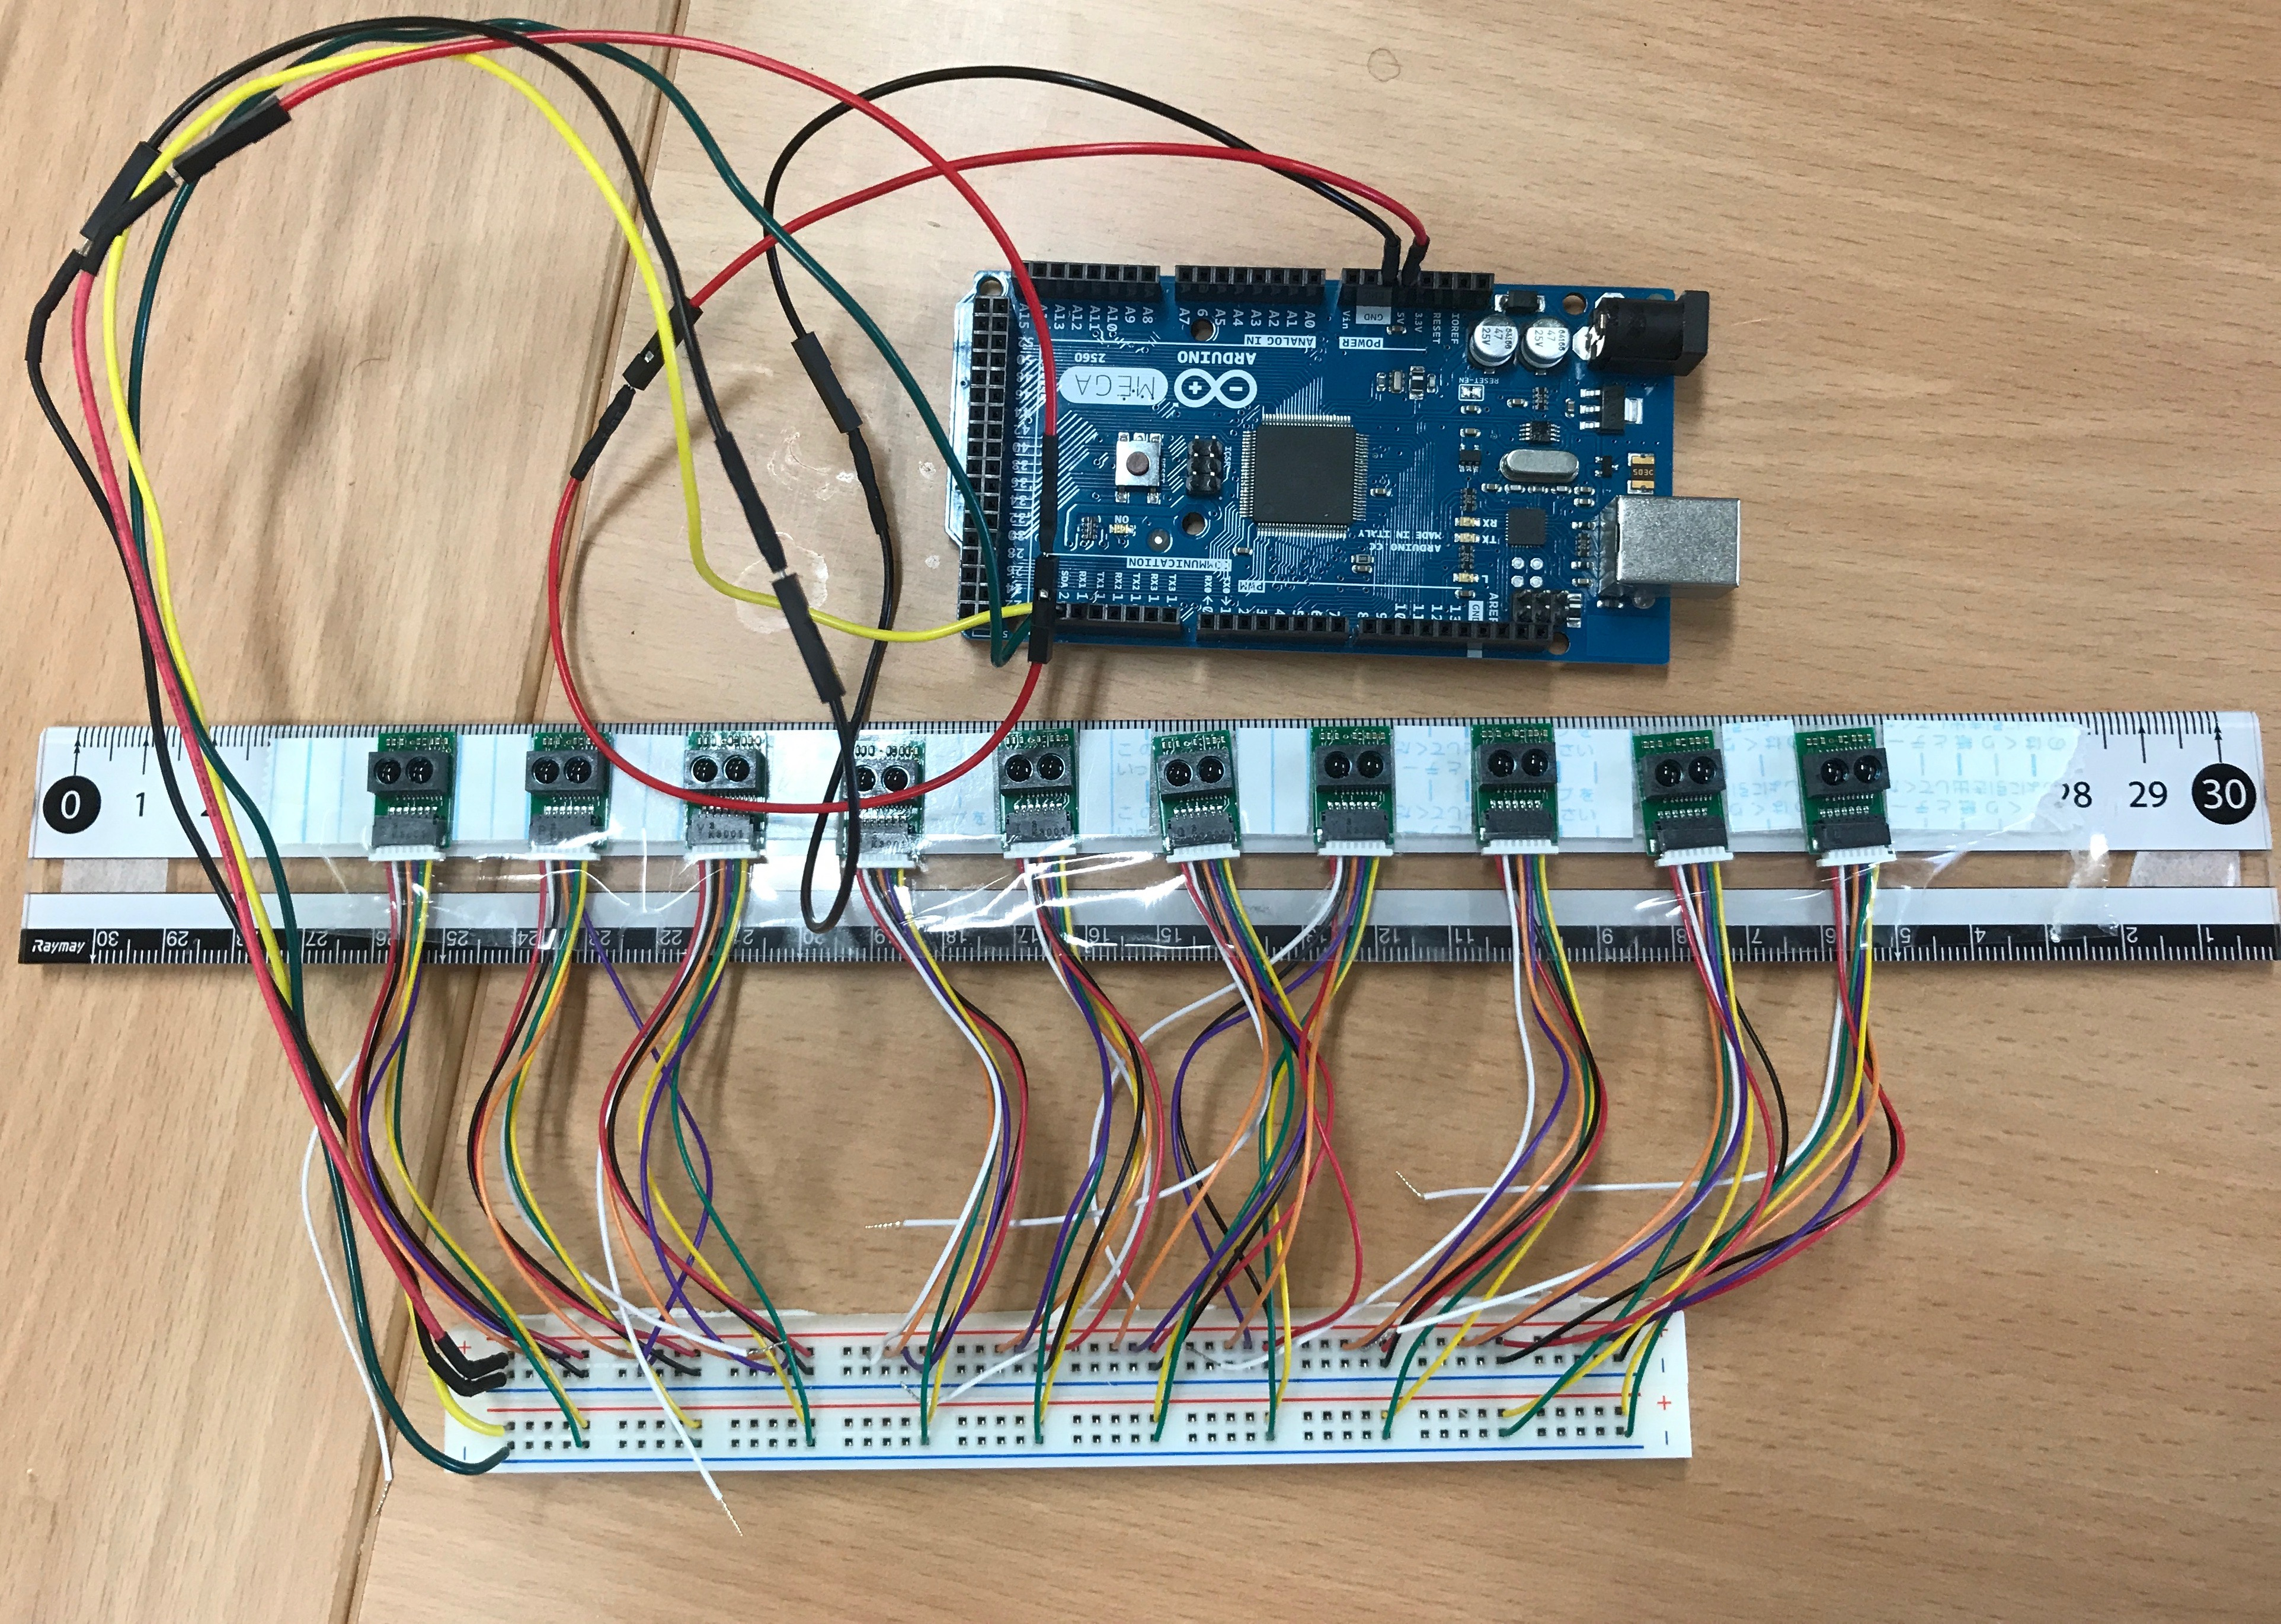
\includegraphics[width = 90mm]{./img/IMG_1794.jpg}
	\end{center}
	\caption{\fixme{プロトタイプその1}}
	\label{img:ig1}
\end{figure}
Arduinoでは、\iic による制御を行い、値をシリアルモニタに送信することだけを行う。したがって、センサのノイズ等の処理は全てソフトウェアで行う。
\subsection{ソフトウェア} 
プログラム言語はPythonを用いた。シリアル通信のためのライブラリとしてPySerial、ポインタを描画するGUIのためのライブラリとしてPyQtを用いた。
膝の位置の計算には、スマートウォッチに搭載した距離センサから指の位置をトラッキングしたXiaoら\cite{Xiao:2018:LOP:3173574.3173669}の研究を参考にした。膝の位置の計算は次のように行う。
\begin{enumerate}
	\item センサからの値を指数平均平滑フィルタを用いて平滑化する。
	\item $y$軸方向の位置をすべての距離センサの最小値とする。
		\begin{eqnarray}
		 	y = min(sensors\_val)
		 	\label{formula:f1}
		\end{eqnarray}
	\item $i$番目の距離センサについて、重み$w_i$を式\ref{formula:f2}のように計算する。ここで、$d$は重み調整の定数である。\SysName では調整の結果$d=2$としている。
		\begin{eqnarray}
			w_i = \cfrac{1}{y_i - y + d}
		\label{formula:f2}
	\end{eqnarray}
	\item $w_i$から、$x$座標を式\ref{formula:f3}のように計算する。
		\begin{eqnarray}
		 	x =\cfrac{\sum iw_i}{\sum w_i}
		 	\label{formula:f3}
		\end{eqnarray} 
	\item ($x,y$)を指数平均平滑フィルタを用いて平滑化する。
	\item ($x,y$)を実際のディスプレイの画面サイズに合わせてマッピングする。
\end{enumerate}
使用者はあらかじめ上下左右方向にキャリブレーションを行い、膝の可動範囲の限界を記録し、これを元に6.のマッピングが行われる。

\subsection{プロトタイプ1の問題点}\subsecLabel{proto1_problem}
実装を行なったプロトタイプを机の裏に設置し、自由なポインタの操作ができるか試みた。キャリブレーション次第では膝を静止させた時にポインタも静止するが、多くの場合は膝を静止させているにも関わらずポインタは左右に振れるなどした。センサからの値を観察したところ、\fixme{膝がかかっていない部分の値}が激しく上下していることがわかった。原因として、以下のようなものが挙げられた。
\begin{enumerate}
	\item アプリケーションノートに、移動物体に対する正しいセンサの設置方向に関する記述があり、センサの設置方向が正しくない可能性がある。
	\item センサのコネクタのピンが細いため、ブレッドボード接続をしたことにより接触不良を起こしている。
	\item 床の色が黒く、赤外線を吸収し正しく距離を計測できていない。
	\item \fixme{センサの設置部分が小さく、膝が範囲外に飛び出してしまう}
\end{enumerate}
\section{プロトタイプ2}
\refSubsec{proto1_problem}であげた問題を解決するために、プロトタイプに改良を行った。1.について、すべてのセンサを90度左回転させて設置した。また同時に4.について、左右方向に膝を傾けた時にどれくらいの範囲を動くかを測定し、必要なセンサのカバー範囲を推定した。測定の結果、におよそ20〜30\si{cm}の長さが必要であるとわかった。このことから、センサの間隔を11\si{mm}から30\si{mm}に変更した。



\chapter{実験:膝によるマウスカーソル操作の性能評価} \chaLabel{exp}
本章では,製作したプロトタイプを用いて膝によるマウスカーソル操作の特徴について実験を行う.
\section{目的}
本実験では,膝によるマウスカーソル操作をフィッツの法則に当てはめて,その特徴を明らかにする.
\section{評価方法}
実験の評価は,フィッツの法則\cite{fitts}を用いて行う.フィッツの法則は,式\ref{formula:fitts}によって表される.
\begin{eqnarray}
	MT = a + b\log_2{(D/W + 1)}
	\label{formula:fitts}
\end{eqnarray}
式\ref{formula:fitts}に用いられている各係数は以下の通りである.
\begin{itemize}
	\item {$MT$(Moving Time): }フィッツの法則から推定される,ポインティングするターゲットを選択するまでにかかる時間
	\item {$a,b$: }ユーザと装置に依存する定数
	\item {$D$: }ポインタがある場所からポインティングするターゲットまでの距離(ターゲット間距離)ここではターゲットが配置されている円の直径に近似する
	\item {$W$: }選択するポインティングするターゲットの幅
	\item { $\log_2{(D/W + 1)}$ [bit]: } 課題の困難度を表す数値\ Index of Difficulty(ID)と呼ばれる
\end{itemize}
IDが高くなればなるほど,それだけポインティングが難しくなり,MTも大きくなる.
性能の評価にはIDから課題を達成するのに要した時間を割った値(Throuput, TP)が用いられる.TPは以下の式で表される.
\begin{eqnarray}
	TP = \cfrac{ID}{MT}
	\label{formula:fitts}
\end{eqnarray}
\section{実験手順}
実験には,ISO9241-411に記載されている,マルチディレクショナルポインティングタスクに基づいて製作したプログラムを使用した.\refImg{mdpt}はそのプログラムである.
参加者は円周上に配置された13個のターゲットを,0から13の順に選択する.選択するべきターゲットは水色で示され,それ以外のターゲットは背景と同じ色で表される.ターゲットを1回選択することを1試行と数え,はじめに0番のターゲットを選択することを除いた13試行を1タスクと数える.膝を動かしてポインタを操作し,ターゲットとポインタが重なった時に選択を行う.本プログラムでは,選択操作は足ではなくキーボード上のEnterキーで行うようプログラムされている.
実験条件として,ターゲット幅($W$)とターゲット間距離($D$)を次のように変化させた.
\img{htbp}{1.0}{mdpt.png}{使用したプログラム}{mdpt}
\begin{itemize}
	\item $D$: 2.0,5.0,8.0 (インチ)
	\item $W$: 0.5,1.0,1.5 (インチ)
\end{itemize}
これにより得られる,以下の9つのIDの条件を1タスクずつ行う.これを1セッションと数える.
\begin{itemize}
	\item $ID = $: \{1.22, 1.59, 2.12, 2.32, 2.59, 2.66, 3.17,  3.46, 4.09\}
\end{itemize}
実験は両膝について3セッションずつ行うものとし,片膝について行うことを1ピリオドと数える.したがって,参加者1人につき,2ピリオド(左右の膝)$\times$13(ターゲット数)$\times$9(条件)$\times$3(セッション)=702試行を行う.試行ごとに,ターゲット選択に要した時間を収集した.1セッション終了ごとに3分間,1ピリオド終了後に10分間の休憩時間を設けた.
参加者はセッションの開始前にプロトタイプを設置した机の前に座り,膝を動かすことができる範囲を決定するためのキャリブレーションを行う.したがって,実験全体では6回キャリブレーションを行う.ピリオドの最初のセッションでは,キャリブレーション後に練習時間を5分設けた.

2ピリオド終了後にアンケートを行った.アンケートは操作の使いやすさ,快適さ,スムーズさ,肉体的難しさ,精神的難しさと腹部,太もも,ふくらはぎ,足の疲労感を5点リッカート尺度で評価するものとした.

本実験には3名が参加した.全て男性であり,年齢はそれぞれP1:22歳,P2:24歳,P3:22歳である.P1,P3は左膝・右膝,P2は右膝・左膝の順でそれぞれ実験を行なった.
\section{収集データ}
解析のために収集したデータは次のとおりである.
\begin{itemize}
	\item 試行ごとのターゲットの選択に要した時間
	\item その試行でターゲット選択が正しくできたかを表すフラグ
\end{itemize}


\section{実験結果}
\refImg{exp_left}は左膝の,\refImg{exp_right}は右膝の実験結果を表す.横軸は式\ref{formula:fitts}におけるID,縦軸は選択時間であり,グラフには各参加者の選択時間と,選択時間を元に線形回帰で求めた直線が描かれている.
\img{htbp}{1.0}{left.pdf}{左膝の選択時間とそのモデル}{exp_left}
\img{htbp}{1.0}{right.pdf}{右膝の選択時間とそのモデル}{exp_right}
\refImg{exp_error}は両膝のエラー率を表す.横軸は参加者であり,縦軸はエラー率が百分率で表される.グラフには参加者ごとにセッション1,2,3のエラー率が棒グラフで表され,全セッションの平均エラー率が折れ線グラフで表されている.全参加者のエラー率の平均は,左膝で1.14\%,右膝で1.71\%であった.
%今回の実験では,全参加者のエラー率の平均が,左膝で1.14\%,右膝で1.71\%であり,これはVellosoら\cite{velloso:hal-01599657}やHorodniczyら\cite{Horodniczy:2017:FHE:3025453.3025625}が行なった実験よりも低い値を得た.
\img{htbp}{0.9}{error.pdf}{両膝のエラー率}{exp_error}

\refImg{exp_tp}は参加者ごとに左膝,右膝のスループットを計算した結果である.縦軸はスループットの値で,横軸は3人の参加者と平均を表している.スループットの平均は,左膝で$1.497$[bit/s],右膝で$1.540$[bit/s]であった.t検定を行なったところ,左右の膝のスループットに有意な差はなかった($t=-0.151, df=4$).
\img{htbp}{1.0}{tp.pdf}{両膝のスループット}{exp_tp}
表\ref{tab:anche}にアンケートの結果を示す.
\begin{table}[]
	\begin{center}
		\caption{アンケートの結果}
		\begin{tabular}{|c|c|c|c|c|}
		\hline 
	   		& P1 & P2 & P3 & 平均   \\ \hline
			\begin{tabular}{c}操作の使いやすさ\\ (1: 使いにくい - 5:使いやすい)\end{tabular}  & 4  & 4  & 3  & 3.67 \\ \hline
			\begin{tabular}{c}操作の快適さ\\ (1: 快適でない- 5:快適である)\end{tabular}  & 4  & 3  & 3  & 3.33 \\ \hline
			\begin{tabular}{c}操作のスムーズさ\\ (1: スムーズでない - 5:スムーズである)\end{tabular}  & 4  & 3  & 3  & 3.33 \\ \hline
			\begin{tabular}{c}肉体的な難しさ\\ (1: 簡単である - 5:難しい)\end{tabular}  & 3  & 1  & 4  & 2.67 \\ \hline
			\begin{tabular}{c}精神的な難しさ\\ (1: 簡単である - 5:難しい)\end{tabular}  & 2  & 1  & 2  & 1.67 \\ \hline
			\begin{tabular}{c}腹部の疲労感\\(1: 疲れていない - 5:疲れている)\end{tabular}& 1  & 1  & 1  & 1.00 \\ \hline
			\begin{tabular}{c}太ももの疲労感\\(1: 疲れていない - 5:疲れている)\end{tabular}& 4  & 1  & 3  & 2.67 \\ \hline
			\begin{tabular}{c}ふくらはぎの疲労感\\(1: 疲れていない - 5:疲れている)\end{tabular}& 3  & 1  & 2  & 2.00 \\ \hline
			\begin{tabular}{c}足の疲労感\\(1: 疲れていない - 5:疲れている)\end{tabular}& 4 & 1  & 3  & 2.67 \\ \hline
		
		\end{tabular}
		\label{tab:anche}

	\end{center}
	
\end{table}
≈

\chapter{今後の展望}\chaLabel{discussion}
本章では,プロトタイプの既知の問題点に対する今後の展望について述べる.

今回のプロトタイプの設計は,直定規に距離センサを貼り付けたため,直線的な形状となった.しかし,膝を左右に傾ける時,膝の運動は直線運動ではなく円弧に近い運動をする.そのため膝がハードウェアの両端付近にある場合と中心付近にある場合とでは,ユーザが水平にカーソルを移動するとき,上下にカーソルがずれてしまう問題が発生する.加えて,ユーザの足の長さによって描く円弧の半径は異なると考える.このことから,膝の運動のユーザ間での違いについてより詳細な分析を行い,その結果からハードウェアの形状を再設計する必要がある.

%ハードウェアは直線形状ではなく円弧に近い形にする必要があり,さらにその形状も,ユーザによって簡単に変えることができるような設計が求められる.そのために,膝の運動のユーザ間での違いについてより詳細な分析も必要となる.

また,今回のプロトタイプでは距離センサを10個をそれぞれ30\si{mm}の間隔で配置した.この設計について,距離センサの数や配置の間隔を増減させた時にも同様なマルチディレクショナルポインティングタスクの実験を行うことで,最適な設計を導く.
\chapter{アプリケーション例}
\chapter{実験2:実際のアプリケーションを用いた評価}
(ここは時間があったら)
\chapter{結論}
\chapter*{謝辞}
\addcontentsline{toc}{chapter}{\numberline{}謝辞}




%図表には番号と説明(caption)を付け、文章中で参照する。表
%\ref{table:fundamental_data_type}と図\ref{figure:sample}はそれぞれ表と図
%の例である。表の説明は上に、図の説明は下に書くことが多い。図の挿入に用い
%るパッケージについては使用環境に合わせて自由に選択してほしい。

%\begin{table}[hbt]
%\caption{表の例}
%\label{table:fundamental_data_type}
%\begin{center}
%\begin{tabular}{| c | r | r | r | r |}
%\hline
%年 度 & 1年次 & 2年次 & 3年次 & 4年次 \\
%\hline
%1995 & 85 & 92 & 86 & 88 \\
%1996 & 83 & 89 & 90 & 102 \\
%1997 & 88 & 87 & 91 & 112 \\
%1998 & 144 & 93 & 90 & 115 \\
%\hline
%\end{tabular}
%\end{center}
%\end{table}
%\medskip

%\begin{figure}[htbp]
%\begin{center}
%\includegraphics[width=3cm]{sample.eps}
%\psfig{file=sample.eps,scale=0.6}
%\epsfile{file=sample.eps,scale=0.6}
%\end{center}
%\caption{図の例}
%\label{figure:sample}
%\end{figure}





\newpage

\addcontentsline{toc}{chapter}{\numberline{}参考文献}
\renewcommand{\bibname}{参考文献}

%% 参考文献に jbibtex を使う場合
\bibliographystyle{junsrt}
\bibliography{ref}
%% [compile] jbibtex sample; platex sample; platex sample;

%% 参考文献を直接ファイルに含めて書く場合
%\begin{thebibliography}{1}
%\bibitem{RakRak}
%野寺隆志.
%\newblock 楽々 \LaTeX.
%\newblock 共立出版, 1990.

%\bibitem{JiyuuJizai}
%磯崎秀樹.
%\newblock \LaTeX 自由自在.
%\newblock サイエンス社, July 1992.

%\bibitem{bryant-ieeetc86}
%Randal~E. Bryant.
%\newblock Graph-based algorithms for {B}oolean function manipulation.
%\newblock {\em IEEE Transactions on Computers}, Vol. C-35, No.~8, pp. 677--691,
%  August 1986.
%\end{thebibliography}

\end{document}
